\pdfpagewidth=8.5in
\pdfpageheight=11in

\documentclass{sig-alternate}
\usepackage[utf8]{inputenc}
\usepackage[T1]{fontenc}
\usepackage{microtype}

\usepackage{url}
\usepackage{amsmath}
\usepackage{graphicx}
\usepackage{subfigure}
\usepackage{threeparttable}
\usepackage{pdflscape}
\usepackage{array}
\usepackage{color}

\usepackage{flushend}

\clubpenalty = 10000
\widowpenalty = 10000
\displaywidowpenalty = 10000

\begin{document}

\conferenceinfo{MSR}{'15, May 16 – 17, 2015, Florence, Italy}
\CopyrightYear{2015}
\crdata{978-1-4503-2863-0/14/05}

\title{Generating the Blueprints of the Java Ecosystem}

\numberofauthors{5}

\def\aueb{\textsuperscript{*}}
\def\columbia{\textsuperscript{\ddag}}
\def\run{\textsuperscript{\dag}}

\author{
  Vassilios Karakoidas\aueb \and Dimitris Mitropoulos\columbia \and Panos Louridas\aueb \and Georgios Gousios\run \and Diomidis Spinellis\aueb\\
  \begin{tabular}{c}
   \affaddr{\aueb Dept of Management Science and Technology}\\
   \affaddr{Athens University of Economics and Business}\\
   \affaddr{Athens, Greece}\\
   \email{\{bkarak,louridas,dds\}@aueb.gr}\\
  \end{tabular}
  \centering
  \begin{tabular}{cc}
   \affaddr{\run Department of Digital Security} & \affaddr{\columbia Computer Science Department}\\
   \affaddr{Radboud University Nijmegen} & \affaddr{Columbia University}\\
   \affaddr{Nijmegen, the Netherlands} & \affaddr{New York, United States}\\
   \email{georgios@cs.ru.nl} & \email{dimitro@cs.columbia.edu}\\
  \end{tabular}
}

\maketitle
\begin{abstract}

\end{abstract}

\category{D.2.4}{Software Engineering}{Software/Program Verification}[Statistical methods]

\terms{Static Analysis, Software Ecosystems.}

\keywords{JDepend, Software Metrics, Chidamber and Kemerer.}

\section{Introduction}
\label{sec:intro}

Software metrics provide a means to extract useful and measurable information about the structure of a software system. Since software artifacts consist of digital data, many of their aspects are easily measured. This explains why the first metrics like {\sc loc} (Lines of Code) and {\sc cloc} (Comment Lines of Code) appeared very early. Over the years, a wealth of different metrics have appeared in the literature. Furthermore, some of them, like Chidamber and Kemerer's~\cite{CHKE94} and those presented by Lorenz et al.~\cite{LOKI94} can be automatically calculated by static analysis tools. 

In this paper, we present a dataset that contains popular metrics, focusing on providing calculation for a large collection of the Java ecosystem. For this purpose we selected the maven~\cite{MAVEN} repository. The tools that were used are the \textit{ckjm} \cite{Spi05g}, \textit{jdepend}~\cite{JDEPEND}, and \textit{clmt}~\cite{SGKL09}.

% dimitro@bkarak: provide corresponding refs. Also you need to bulk this up. A paragraph referring to what we did. e.g "In this paper we present a dataset produced by applying three tools on all versions of a snapshot of the Maven repository. [...]".

\section{Dataset Construction Process}
\label{sec:data}

% dimitro@bkarak: This section *does not* present the dataset. It presents Maven. You should rename the section to "Dataset Construction Process" and merge it with the upcoming one. It should go like this: 1) We got this snapshot and 2) applied these three tools to create what you see in the next section. You'll present the experiment and *advertise* the effort.

Maven is a build automation tool used primarily for Java projects, and it is hosted by the Apache Software Foundation~\cite{MAVEN}. To describe the software project being built, its dependencies on other libraries, and the build order Maven uses {\sc xml}. The repository contains more than 400,000 {\sc jar}s, in a variety of languages that are all using the {\sc jvm} platform as basis. These languages include Java, Clojure, Groovy, and Scala.

Initially, a snapshot (January 2012) of the Maven repository was downloaded locally. The repository contains various projects and their releases. A project version can be uniquely identified by the following triplet: {\it group id}, {\it artifact id} and {\it version}. The Maven repository contains several versions of each project.

All versions were filtered out and only the latest was kept. For each version in the Maven repository, each binary {\sc jar} file is accompanied by another {\sc jar}, which contains the source code. Table \ref{tbl:oss-size-metrics} presents several size metrics regarding the final version corpus. It included 12,959 projects, with more than 110 million lines of code. Overall the dataset contains almost 33 million unique measurements.

\begin{table}
\centering
\caption{The selected Maven projects' size metrics}
\label{tbl:oss-size-metrics}
\begin{tabular}{l r}
 \hline
\textbf{Metric} & \textbf{Value}\\
\hline
Project Count & 11,365\\
File Count & 604,821\\
Module Count & 72,302\\
Lines of Code & 110,156,703\\
Source Lines of Code & 61,246,807\\
Comment Lines of Code & 36,696,217\\
Number of Classes & 499,588\\
Number of Interfaces & 89,145\\
Number of Enumerations & 12,732\\
Measurement Count & 32,844,836\\
\hline
\end{tabular}
\end{table}

Table~\ref{tbl:selected-metrics} presents the key metrics that are calculated and stored in the dataset. Each tool focuses on a different aspect of a software system; \textit{ckjm} focuses on object-oriented design metrics, \textit{jdepend} on package design, while \textit{clmt} focuses on program size metrics. Several metrics are calculated by more than one tools in this dataset, like \textit{cyclomatic complexity}, which is calculated by both \textit{clmt} and \textit{ckjm}. Both calculation are stored and provided by the dataset.Three tools were selected.

\begin{itemize}
  \item \textbf{CKJM-ext} \textit{(ckjm)}~\cite{Spi05g} is an open source tool that was developed by Diomidis Spinellis and then extended by Marian Jureczko. It calculates many software complexity metrics, including the \textit{Chidamber and Kemmerer} set of object-oriented metrics \cite{CHKE94}. The version of the tool that we used for this experiment can be found in github~\cite{CKJM}.

  \item \textbf{JDepend} \textit{(jdep)}~\cite{JDEPEND} is a tool that analyses {\sc jar} files that contain compiled Java classes and calculates a series of design metrics.

  \item \textbf{CLMT} \textit{(clmt)}~\cite{SGKL09} stands for \textit{cross-language metric tool} and analyses the source code of several languages in order to calculate a series of size metrics.
\end{itemize}

\begin{table}
\centering
\caption{Key Metrics}
\label{tbl:selected-metrics}
\begin{tabular}{l l}
 \hline
\multicolumn{2}{l}{\textit{\textbf{Class Design}}}\\
\hline
Depth Of Inheritance Tree & \textit{ckjm}\\
Coupling Between Objects & \textit{ckjm}\\
Weighted Methods Per Class & \textit{ckjm}\\
Response For Class & \textit{ckjm}\\
Lack Of Cohesion In Methods & \textit{ckjm}\\
Number Of Children & \textit{ckjm}\\
Attribute Hiding Factor & \textit{clmt}\\
Coupling Between Methods & \textit{ckjm}\\
Average Method Complexity & \textit{ckjm}\\
Cohesion Among Methods of Class & \textit{ckjm}\\
Data Access Metric & \textit{ckjm, clmt}\\
Inheritance Coupling & \textit{ckjm}\\
Lack Of Cohesion In Methods3 & \textit{ckjm}\\
Measure Of Aggregation & \textit{ckjm}\\
Measure Of Functional Abstraction & \textit{ckjm}\\
Number of Attributes & \textit{clmt}\\
Method Hiding Factor & \textit{clmt}\\
\hline
\multicolumn{2}{l}{\textit{\textbf{Method Design}}}\\
\hline
Number of Method Parameters & \textit{clmt}\\
Number of Methods & \textit{clmt, ckjm}\\
McCabe Cyclomatic Complexity & \textit{ckjm, clmt}\\
\hline
\multicolumn{2}{l}{\textit{\textbf{Package Design}}}\\
\hline
Number of Concrete Classes & \textit{jdep}\\
Afferent Couplings & \textit{jdep, ckjm}\\
Efferent Couplings & \textit{jdep, ckjm}\\
Instability & \textit{jdep}\\
Abstractness & \textit{jdep}\\
Distance Main Sequence & \textit{jdep}\\
\hline
\multicolumn{2}{l}{\textit{\textbf{Program Size Metrics}}}\\
\hline
Number of Classes & \textit{clmt, ckjm, jdep}\\
Number of Enumerations & \textit{clmt, ckjm}\\
Number of Interfaces & \textit{clmt, ckjm}\\
Module Count & \textit{clmt, ckjm}\\
Comments Lines Of Code & \textit{clmt}\\
Lines Of Code & \textit{clmt, ckjm}\\
Source Lines Of Code & \textit{clmt}\\
Function Oriented Code & \textit{clmt}\\
DSL Usage Count & \textit{clmt}\\
File Count & \textit{clmt}\\
\hline
\end{tabular}
\end{table}

\section{Database Structure}
\label{sec:db}

Figure~\ref{fig:database-schema} illustrates the database schema. The data are stored in a straightforward manner. The database schema consists of five tables; \textit{measurement}, \textit{category}, \textit{identifiers}, \textit{measurement\_type}, and \textit{project}. The central table is \textit{measurement}, which holds the actual measurement values. The other tables are used as normalisation tables.

Metrics are divided in six categories that defined its scope; \textit{module}, \textit{class}, \textit{method}, \textit{code unit}, and \textit{project-wide}. These values are stored in \textit{category} table.

The descriptive names for each metric are stored in the \textit{measurement\_type} table. There are 65 metrics available in the dataset. The names are composed by the actual metric name and the tool that was used to calculate them e.g. \textit{McCabe\_clmt} denotes that the metric name is the McCabe cyclomatic complexity from the clmt tool, while \textit{McCabe\_ckjm} means that it is the same metric calculated by the ckjm tool.

Filenames, method, class and package names along with other identifiers are stored in the \textit{identifiers} table. Note that each measurement has a related filename and a related identifier that points to the software element that is related e.g. the \textit{afferent coupling} metric for the module in the directory ``com/scalagent/jmx'' is related with the identifier \textit{com.scalagent.jmx}.

Finally the table \textit{project} contains the related project identifiers, extracted from the maven repository.

\begin{figure*}
\centering
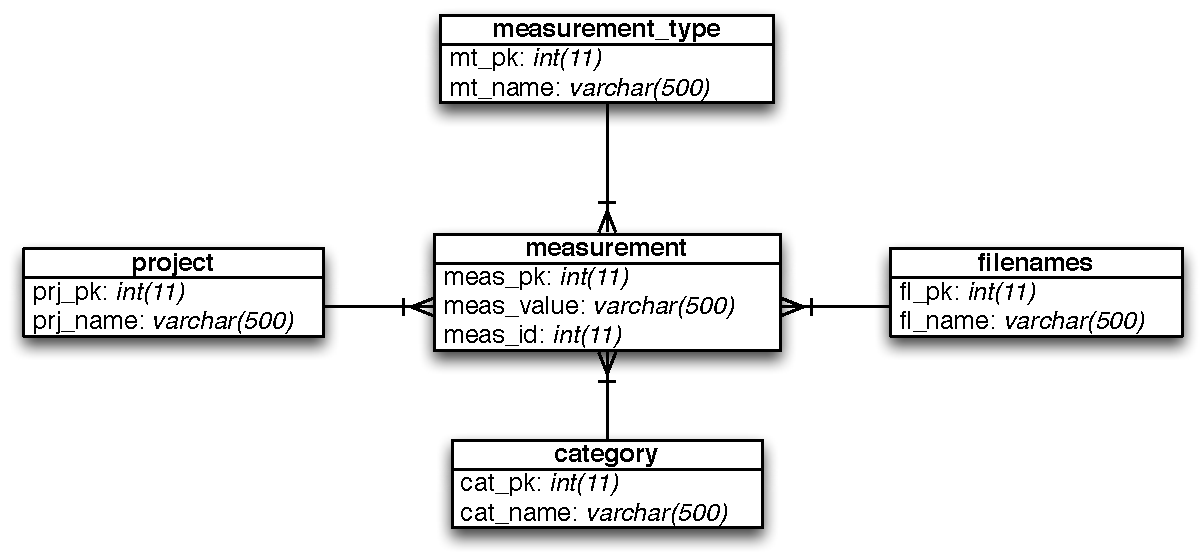
\includegraphics[scale=0.7]{database-schema}
\caption{The database schema}
\label{fig:database-schema}
\end{figure*}

\section{Experimenting with the Dataset}
\label{sec:dsl}

The Java platform exists for more than a decade and provides a development environment for several application areas, such as web, grid computing, and traditional client-server applications. The official development environment of the Java platform is released by Oracle and is widely-known as the Java Standard Edition {\sc sdk}. The process of development and innovation in the Java ecosystem is built around a community, that writes proposals of features, known as Java Specification Requests ({\sc jsr}s), which are supported by prototype implementations.

In the literature, it is suggested that {\sc dsl}s are used to reduce software development cost, by introducing domain efficiency \cite{MHS05}. This thesis focuses on practical research aspects as well as with the theoretical ones; thus the first problem that needs to be examined, is to measure the adoption of {\sc dsl}s in software projects. In addition, the average number of {\sc dsl}s usually used in a software project needs to be investigated.

The methodology was the following; A set of standard {\sc dsl} application libraries was identified, and the source was scanned for specific \textit{import} statements e.g. \textit{java.util.regex}, which indicated that the standard package that implements regular expressions was used, thus regular expressions were used. If a package is detected in the source code, then the project will be tagged that it uses one (1) {\sc dsl}. Consequently, if a project has {\sc dsl} count four (4), then it means that four (4) different application libraries were detected during the source code scan. Table \ref{tbl:dsl-list} lists the selected {\sc dsl}s application libraries. Note that all these libraries are included as part of the Java {\sc sdk}.

\begin{table}
\centering
\caption{List of selected DSL application libraries}
\label{tbl:dsl-list}
\begin{tabular}{l l}
 \hline
\textbf{DSL} & \textbf{Java Package}\\
\hline
Regular Expressions & \verb|java.util.regex|\\
XML & \verb|javax.xml|, \verb|org.w3c| and \verb|org.xml|\\
SQL & \verb|java.sql| and \verb|javax.sql|\\
XPath & \verb|java.xml.xpath|\\
XSLT & \verb|javax.xml.transform|\\
RTF & \verb|javax.swing.text.rtf|\\
HTML & \verb|javax.swing.text.html|\\
\hline
\end{tabular}
\end{table}

The initial goal of this experiment was to provide quantifiable results that are indicative regarding the usage of each {\sc dsl}, thus only files containing Java code were taken into account. Build files or other resources that may contain {\sc dsl}s were not included. One final assumption was also made; if {\sc xpath} or {\sc xslt} were found in the source code, then the project would be marked that it also uses {\sc xml}, since those two languages are used for query and transformations on {\sc xml} {\sc dom} trees.

\begin{table}
\centering
\caption{Popular DSL Usage Combinations}
\label{tbl:dsl-top-usage}
\begin{tabular}{l r}
 \hline
\textbf{DSLs} & \textbf{Count}\\
\hline
XML & 1,561\\
Regex & 909\\
SQL & 493\\
XML, XSLT & 475\\
Regex, XML, XSLT & 158\\
Regex, XML & 303\\
SQL, XML & 162\\
Regex, SQL & 116\\
Regex, SQL, XML, XSLT & 80\\
Regex, SQL, XML & 71\\
SQL, XML, XSLT & 54\\
XML, XPath & 50\\
XML, XPath, XSLT & 39\\
Regex, XML, XPath, XSLT & 38\\
HTML & 23\\
Regex, XML, XPath & 20\\
Regex, SQL, XML, XPath, XSLT & 18\\
SQL, XML, XPath, XSLT & 11\\
HTML, Regex, XML & 10\\
HTML, XML & 10\\
\hline
\end{tabular}
\end{table}

\section{Limitations}
\label{sec:limit}

\section{Related Work}
\label{sec:rel}

The Maven ecosystem has been previously analyzed by Raemaekers et al.~\cite{RDV13} to produce the {\it Maven dependency dataset}. Apart from basic information like individual methods, classes, packages and lines of code for every {\sc jar}, this dataset also includes a database with all the connections between the aforementioned elements. In publication \cite{MKLGS14}, Mitropoulos et al. also experimented in a similar way, by running the FindBugs~\cite{HP04} tool on a large part of the maven repository. Our work differs from these two approaches since it presents the metrics calculated by the three aforementioned tools; \textit{ckjm}, \textit{jdepend}, and \textit{clmt}.

\section{Conclusions}
\label{sec:conc}

\section{Availability}

The dataset and the source code of this publication, along with some utility scripts are available at \url{https://github.com/bkarak/data_msr2015}.

\bibliographystyle{abbrv}
\bibliography{msr}

\end{document}
